\subsection{MSVC: x86}

Aqui está o a saída em assembly (MSVC 2010):

\lstinputlisting{patterns/04_scanf/3_checking_retval/ex3_MSVC_x86.asm}

\myindex{x86!\Registers!EAX}
A função que chamou (\main) precisa do resultado da função chamada (\scanf),
então a função chamada retorna esse valor no registrador \EAX.

\myindex{x86!\Instructions!CMP}
Nós verificamos com a ajuda da instrução \TT{CMP EAX, 1} (\IT{CoMParar}). Em outras palavras, comparamos o valor em \EAX com 1.

\myindex{x86!\Instructions!JNE}
O jump condicional \JNE está logo depois da instrução \CMP. \JNE significa \IT{Jump if Not Equal} ou seja, ela desvia se o valor não for igual ao comparado.

Então, se o valor em \EAX não é 1, a \ac{CPU} vai passar a execução para o endereço contido no operando de \JNE, no nosso caso \TT{\$LN2@main}.
Passando a execução para esse endereço resulta na \ac{CPU} executando \printf com o argumento \TT{What you entered? Huh?}.
Mas se tudo estiver correto, o jump condicional não será efetuado e outra chamada do \printf é executada, com dois argumentos: \TT{`You entered \%d...'} e o valor de \TT{x}.

\myindex{x86!\Instructions!XOR}
\myindex{\CLanguageElements!return}
Como nesse caso o segundo \printf() não tem que ser executado, tem um \JMP precedendo ele (jump incondicional).
Ele passa a execução para o ponto depois do segundo \printf e logo antes de \TT{XOR EAX, EAX}, que implementa \TT{return 0}.

% FIXME internal \ref{} to x86 flags instead of wikipedia
\myindex{x86!\Registers!\Flags}
Então, podemos dizer que comparar um valor com outro é geralmente realizado através do par de instruções \CMP/\Jcc, onde \IT{cc} é código condicional.
\CMP compara dois valores e altera os registros da \ac{CPU} (flags)\footnote{\ac{TBT}: x86 flags, see also: \href{http://go.yurichev.com/17120}{wikipedia}.}.
\Jcc checa esses registro e decide passar a execução para o endereço específico contido no operando ou não.

\myindex{x86!\Instructions!CMP}
\myindex{x86!\Instructions!SUB}
\myindex{x86!\Instructions!JNE}
\myindex{x86!\Registers!ZF}
\label{CMPandSUB}
Isso pode parecer meio paradoxal, mas a instrução \CMP é na verdade \SUB (subtrair).
Todo o conjunto de instruções aritiméticas alteram os registros da \ac{CPU}, não só \CMP.
Se compararmos 1 e 1, $1-1$ é 0 então \ZF (zero flag) será acionado (significando que o último resultado foi zero).
Em nenhuma outra circunstância \ZF pode ser acionado, exceto quando os operandos forem iguais.
\JNE verifica somente o ZF e desvia só não estiver acionado.
\JNE é na verdade um sinônimo para \JNZ (jump se não zero).
\JNE e \JNZ são traduzidos no mesmo código de operação.
Então, a instrução CMP pode ser substituida com a instrução \SUB e quase tudo estará certo, com a diferença de que \SUB altera o valor do primeiro operando.
\CMP é \SUB sem salvar o resultado, mas afetando os registros da \ac{CPU}.

\subsection{MSVC: x86: IDA}

\PTBRph{}

% TODO translate: \input{patterns/04_scanf/3_checking_retval/olly_PTBR.tex}

\clearpage
\subsection{MSVC: x86 + Hiew}
\myindex{Hiew}

Esse exemplo também pode ser usado como uma maneira simples de exemplificar o patch de arquivos executáveis.
Nós podemos tentar rearranjar o executável de forma que o programa sempre imprima a saída, não importando o que inserirmos.

Assumindo que o executavel está compilado com a opção \TT{/MD}\footnote{isso também é chamada ``linkagem dinâmica''}
(\TT{MSVCR*.DLL}), nós vemos a função main no começo da seção \TT{.text}.
Vamos abrir o executável no Hiew e procurar o começo da seção \TT{.text} (Enter, F8, F6, Enter, Enter).

Nós chegamos a isso:

\begin{figure}[H]
\centering
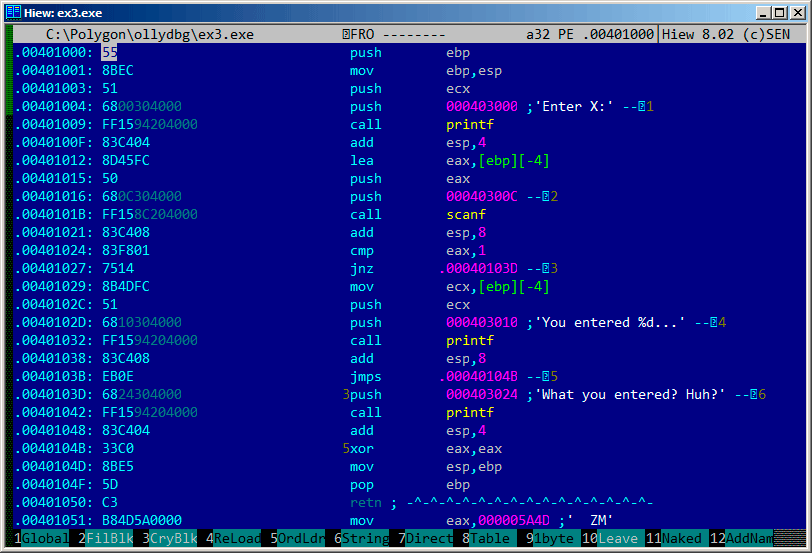
\includegraphics[scale=\FigScale]{patterns/04_scanf/3_checking_retval/hiew_1.png}
\caption{\PTBRph{}}
\label{fig:scanf_ex3_hiew_1}
\end{figure}

Hiew encontra strings em \ac{ASCIIZ} e as exibe, como faz com os nomes de funções importadas.

\clearpage
Mova o cursor para o endereço \TT{.00401027} (onde a instrução \TT{JNZ}, que temos de evitar, está localizada), aperte F3 e então digite \q{9090} (que significa dois \ac{NOP}s):

\begin{figure}[H]
\centering
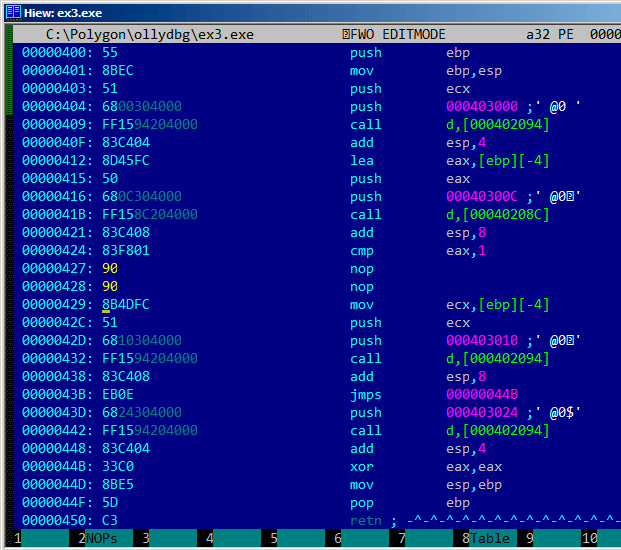
\includegraphics[scale=\FigScale]{patterns/04_scanf/3_checking_retval/hiew_2.png}
\caption{PTBRph{}}
\label{fig:scanf_ex3_hiew_2}
\end{figure}

Então aperte F9 (atualizar). Agora o executável está salvo no disco. Ele executará da maneira que nós desejávamos.

Duas instruções \ac{NOP} não é a abordagem mais estética.
Outra maneira de rearranjar essa instrução é somente escrever um 0 no operando da instrução jump,
então \INS{JNZ} só avançará para a próxima instrução.

Nós poderíamos também ter feito o oposto: mudado o primeiro byte com \TT{EB} e deixa o segundo byte como está.
Nós teriamos um jump incondicional que é sempre deviado.
Nesse caso, a mensagem de erro seria mostrada todas as vezes, não importando a entrada.

